%% V1.3
%% 2007/01/11
%% by Michael Shell
%% see http://www.michaelshell.org/
%% for current contact information.
%%
%% This is a skeleton file demonstrating the use of IEEEtran.cls
%% (requires IEEEtran.cls version 1.7 or later) with an IEEE journal paper.
%%
%% Support sites:
%% http://www.michaelshell.org/tex/ieeetran/
%% http://www.ctan.org/tex-archive/macros/latex/contrib/IEEEtran/
%% and
%% http://www.ieee.org/



% *** Authors should verify (and, if needed, correct) their LaTeX system  ***
% *** with the testflow diagnostic prior to trusting their LaTeX platform ***
% *** with production work. IEEE's font choices can trigger bugs that do  ***
% *** not appear when using other class files.                            ***
% The testflow support page is at:
% http://www.michaelshell.org/tex/testflow/


%%*************************************************************************
%% Legal Notice:
%% This code is offered as-is without any warranty either expressed or
%% implied; without even the implied warranty of MERCHANTABILITY or
%% FITNESS FOR A PARTICULAR PURPOSE!
%% User assumes all risk.
%% In no event shall IEEE or any contributor to this code be liable for
%% any damages or losses, including, but not limited to, incidental,
%% consequential, or any other damages, resulting from the use or misuse
%% of any information contained here.
%%
%% All comments are the opinions of their respective authors and are not
%% necessarily endorsed by the IEEE.
%%
%% This work is distributed under the LaTeX Project Public License (LPPL)
%% ( http://www.latex-project.org/ ) version 1.3, and may be freely used,
%% distributed and modified. A copy of the LPPL, version 1.3, is included
%% in the base LaTeX documentation of all distributions of LaTeX released
%% 2003/12/01 or later.
%% Retain all contribution notices and credits.
%% ** Modified files should be clearly indicated as such, including  **
%% ** renaming them and changing author support contact information. **
%%
%% File list of work: IEEEtran.cls, IEEEtran_HOWTO.pdf, bare_adv.tex,
%%                    bare_conf.tex, bare_jrnl.tex, bare_jrnl_compsoc.tex
%%*************************************************************************

% Note that the a4paper option is mainly intended so that authors in
% countries using A4 can easily print to A4 and see how their papers will
% look in print - the typesetting of the document will not typically be
% affected with changes in paper size (but the bottom and side margins will).
% Use the testflow package mentioned above to verify correct handling of
% both paper sizes by the user's LaTeX system.
%
% Also note that the "draftcls" or "draftclsnofoot", not "draft", option
% should be used if it is desired that the figures are to be displayed in
% draft mode.
%
\documentclass[10pt,conference]{IEEEtran}

%
% If IEEEtran.cls has not been installed into the LaTeX system files,
% manually specify the path to it like:
% \documentclass[journal]{../sty/IEEEtran}


% Added to solve the error: "! Package babel Error: You haven't defined the language ENGLISH yet."
% Reference: http://www.michaelshell.org/tex/ieeetran/
\makeatletter
\def\markboth#1#2{\def\leftmark{\@IEEEcompsoconly{\sffamily}\MakeUppercase{\protect#1}}%
\def\rightmark{\@IEEEcompsoconly{\sffamily}\MakeUppercase{\protect#2}}}
\makeatother



% Some very useful LaTeX packages include:
% (uncomment the ones you want to load)

\usepackage[english]{babel} % for multilingual support
% \usepackage{babel} % for multilingual support

\usepackage[utf8]{inputenc} % for use utf8


% *** MISC UTILITY PACKAGES ***
%
%\usepackage{ifpdf}
% Heiko Oberdiek's ifpdf.sty is very useful if you need conditional
% compilation based on whether the output is pdf or dvi.
% usage:
% \ifpdf
%   % pdf code
% \else
%   % dvi code
% \fi
% The latest version of ifpdf.sty can be obtained from:
% http://www.ctan.org/tex-archive/macros/latex/contrib/oberdiek/
% Also, note that IEEEtran.cls V1.7 and later provides a builtin
% \ifCLASSINFOpdf conditional that works the same way.
% When switching from latex to pdflatex and vice-versa, the compiler may
% have to be run twice to clear warning/error messages.






% *** CITATION PACKAGES ***
%
%\usepackage{cite}
% cite.sty was written by Donald Arseneau
% V1.6 and later of IEEEtran pre-defines the format of the cite.sty package
% \cite{} output to follow that of IEEE. Loading the cite package will
% result in citation numbers being automatically sorted and properly
% "compressed/ranged". e.g., [1], [9], [2], [7], [5], [6] without using
% cite.sty will become [1], [2], [5]--[7], [9] using cite.sty. cite.sty's
% \cite will automatically add leading space, if needed. Use cite.sty's
% noadjust option (cite.sty V3.8 and later) if you want to turn this off.
% cite.sty is already installed on most LaTeX systems. Be sure and use
% version 4.0 (2003-05-27) and later if using hyperref.sty. cite.sty does
% not currently provide for hyperlinked citations.
% The latest version can be obtained at:
% http://www.ctan.org/tex-archive/macros/latex/contrib/cite/
% The documentation is contained in the cite.sty file itself.






% *** GRAPHICS RELATED PACKAGES ***
%
\ifCLASSINFOpdf
  \usepackage[pdftex]{graphicx}
%  \usepackage[caption=false]{subfig} % Para usar duas ou mais figuras como uma só.
  % declare the path(s) where your graphic files are
  % \graphicspath{{../pdf/}{../jpeg/}}
  % and their extensions so you won't have to specify these with
  % every instance of \includegraphics
  % \DeclareGraphicsExtensions{.pdf,.jpeg,.png}


\else
  % or other class option (dvipsone, dvipdf, if not using dvips). graphicx
  % will default to the driver specified in the system graphics.cfg if no
  % driver is specified.
  % \usepackage[dvips]{graphicx}
  % declare the path(s) where your graphic files are
  % \graphicspath{{../eps/}}
  % and their extensions so you won't have to specify these with
  % every instance of \includegraphics
  % \DeclareGraphicsExtensions{.eps}
\fi
% graphicx was written by David Carlisle and Sebastian Rahtz. It is
% required if you want graphics, photos, etc. graphicx.sty is already
% installed on most LaTeX systems. The latest version and documentation can
% be obtained at:
% http://www.ctan.org/tex-archive/macros/latex/required/graphics/
% Another good source of documentation is "Using Imported Graphics in
% LaTeX2e" by Keith Reckdahl which can be found as epslatex.ps or
% epslatex.pdf at: http://www.ctan.org/tex-archive/info/
%
% latex, and pdflatex in dvi mode, support graphics in encapsulated
% postscript (.eps) format. pdflatex in pdf mode supports graphics
% in .pdf, .jpeg, .png and .mps (metapost) formats. Users should ensure
% that all non-photo figures use a vector format (.eps, .pdf, .mps) and
% not a bitmapped formats (.jpeg, .png). IEEE frowns on bitmapped formats
% which can result in "jaggedy"/blurry rendering of lines and letters as
% well as large increases in file sizes.
%
% You can find documentation about the pdfTeX application at:
% http://www.tug.org/applications/pdftex





% *** MATH PACKAGES ***
%
%\usepackage[cmex10]{amsmath}
% A popular package from the American Mathematical Society that provides
% many useful and powerful commands for dealing with mathematics. If using
% it, be sure to load this package with the cmex10 option to ensure that
% only type 1 fonts will utilized at all point sizes. Without this option,
% it is possible that some math symbols, particularly those within
% footnotes, will be rendered in bitmap form which will result in a
% document that can not be IEEE Xplore compliant!
%
% Also, note that the amsmath package sets \interdisplaylinepenalty to 10000
% thus preventing page breaks from occurring within multiline equations. Use:
%\interdisplaylinepenalty=2500
% after loading amsmath to restore such page breaks as IEEEtran.cls normally
% does. amsmath.sty is already installed on most LaTeX systems. The latest
% version and documentation can be obtained at:
% http://www.ctan.org/tex-archive/macros/latex/required/amslatex/math/





% *** SPECIALIZED LIST PACKAGES ***
%
%\usepackage{algorithmic}
% algorithmic.sty was written by Peter Williams and Rogerio Brito.
% This package provides an algorithmic environment fo describing algorithms.
% You can use the algorithmic environment in-text or within a figure
% environment to provide for a floating algorithm. Do NOT use the algorithm
% floating environment provided by algorithm.sty (by the same authors) or
% algorithm2e.sty (by Christophe Fiorio) as IEEE does not use dedicated
% algorithm float types and packages that provide these will not provide
% correct IEEE style captions. The latest version and documentation of
% algorithmic.sty can be obtained at:
% http://www.ctan.org/tex-archive/macros/latex/contrib/algorithms/
% There is also a support site at:
% http://algorithms.berlios.de/index.html
% Also of interest may be the (relatively newer and more customizable)
% algorithmicx.sty package by Szasz Janos:
% http://www.ctan.org/tex-archive/macros/latex/contrib/algorithmicx/




% *** ALIGNMENT PACKAGES ***
%
%\usepackage{array}
% Frank Mittelbach's and David Carlisle's array.sty patches and improves
% the standard LaTeX2e array and tabular environments to provide better
% appearance and additional user controls. As the default LaTeX2e table
% generation code is lacking to the point of almost being broken with
% respect to the quality of the end results, all users are strongly
% advised to use an enhanced (at the very least that provided by array.sty)
% set of table tools. array.sty is already installed on most systems. The
% latest version and documentation can be obtained at:
% http://www.ctan.org/tex-archive/macros/latex/required/tools/


%\usepackage{mdwmath}
%\usepackage{mdwtab}
% Also highly recommended is Mark Wooding's extremely powerful MDW tools,
% especially mdwmath.sty and mdwtab.sty which are used to format equations
% and tables, respectively. The MDWtools set is already installed on most
% LaTeX systems. The lastest version and documentation is available at:
% http://www.ctan.org/tex-archive/macros/latex/contrib/mdwtools/


% IEEEtran contains the IEEEeqnarray family of commands that can be used to
% generate multiline equations as well as matrices, tables, etc., of high
% quality.


%\usepackage{eqparbox}
% Also of notable interest is Scott Pakin's eqparbox package for creating
% (automatically sized) equal width boxes - aka "natural width parboxes".
% Available at:
% http://www.ctan.org/tex-archive/macros/latex/contrib/eqparbox/





% *** SUBFIGURE PACKAGES ***
%\usepackage[tight,footnotesize]{subfigure}
% subfigure.sty was written by Steven Douglas Cochran. This package makes it
% easy to put subfigures in your figures. e.g., "Figure 1a and 1b". For IEEE
% work, it is a good idea to load it with the tight package option to reduce
% the amount of white space around the subfigures. subfigure.sty is already
% installed on most LaTeX systems. The latest version and documentation can
% be obtained at:
% http://www.ctan.org/tex-archive/obsolete/macros/latex/contrib/subfigure/
% subfigure.sty has been superceeded by subfig.sty.



%\usepackage[caption=false]{caption}
%\usepackage[font=footnotesize]{subfig}
% subfig.sty, also written by Steven Douglas Cochran, is the modern
% replacement for subfigure.sty. However, subfig.sty requires and
% automatically loads Axel Sommerfeldt's caption.sty which will override
% IEEEtran.cls handling of captions and this will result in nonIEEE style
% figure/table captions. To prevent this problem, be sure and preload
% caption.sty with its "caption=false" package option. This is will preserve
% IEEEtran.cls handing of captions. Version 1.3 (2005/06/28) and later
% (recommended due to many improvements over 1.2) of subfig.sty supports
% the caption=false option directly:
%\usepackage[caption=false,font=footnotesize]{subfig}
%
% The latest version and documentation can be obtained at:
% http://www.ctan.org/tex-archive/macros/latex/contrib/subfig/
% The latest version and documentation of caption.sty can be obtained at:
% http://www.ctan.org/tex-archive/macros/latex/contrib/caption/




% *** FLOAT PACKAGES ***
%
%\usepackage{fixltx2e}
% fixltx2e, the successor to the earlier fix2col.sty, was written by
% Frank Mittelbach and David Carlisle. This package corrects a few problems
% in the LaTeX2e kernel, the most notable of which is that in current
% LaTeX2e releases, the ordering of single and double column floats is not
% guaranteed to be preserved. Thus, an unpatched LaTeX2e can allow a
% single column figure to be placed prior to an earlier double column
% figure. The latest version and documentation can be found at:
% http://www.ctan.org/tex-archive/macros/latex/base/



%\usepackage{stfloats}
% stfloats.sty was written by Sigitas Tolusis. This package gives LaTeX2e
% the ability to do double column floats at the bottom of the page as well
% as the top. (e.g., "\begin{figure*}[!b]" is not normally possible in
% LaTeX2e). It also provides a command:
%\fnbelowfloat
% to enable the placement of footnotes below bottom floats (the standard
% LaTeX2e kernel puts them above bottom floats). This is an invasive package
% which rewrites many portions of the LaTeX2e float routines. It may not work
% with other packages that modify the LaTeX2e float routines. The latest
% version and documentation can be obtained at:
% http://www.ctan.org/tex-archive/macros/latex/contrib/sttools/
% Documentation is contained in the stfloats.sty comments as well as in the
% presfull.pdf file. Do not use the stfloats baselinefloat ability as IEEE
% does not allow \baselineskip to stretch. Authors submitting work to the
% IEEE should note that IEEE rarely uses double column equations and
% that authors should try to avoid such use. Do not be tempted to use the
% cuted.sty or midfloat.sty packages (also by Sigitas Tolusis) as IEEE does
% not format its papers in such ways.


%\ifCLASSOPTIONcaptionsoff
%  \usepackage[nomarkers]{endfloat}
% \let\MYoriglatexcaption\caption
% \renewcommand{\caption}[2][\relax]{\MYoriglatexcaption[#2]{#2}}
%\fi
% endfloat.sty was written by James Darrell McCauley and Jeff Goldberg.
% This package may be useful when used in conjunction with IEEEtran.cls'
% captionsoff option. Some IEEE journals/societies require that submissions
% have lists of figures/tables at the end of the paper and that
% figures/tables without any captions are placed on a page by themselves at
% the end of the document. If needed, the draftcls IEEEtran class option or
% \CLASSINPUTbaselinestretch interface can be used to increase the line
% spacing as well. Be sure and use the nomarkers option of endfloat to
% prevent endfloat from "marking" where the figures would have been placed
% in the text. The two hack lines of code above are a slight modification of
% that suggested by in the endfloat docs (section 8.3.1) to ensure that
% the full captions always appear in the list of figures/tables - even if
% the user used the short optional argument of \caption[]{}.
% IEEE papers do not typically make use of \caption[]'s optional argument,
% so this should not be an issue. A similar trick can be used to disable
% captions of packages such as subfig.sty that lack options to turn off
% the subcaptions:
% For subfig.sty:
% \let\MYorigsubfloat\subfloat
% \renewcommand{\subfloat}[2][\relax]{\MYorigsubfloat[]{#2}}
% For subfigure.sty:
% \let\MYorigsubfigure\subfigure
% \renewcommand{\subfigure}[2][\relax]{\MYorigsubfigure[]{#2}}
% However, the above trick will not work if both optional arguments of
% the \subfloat/subfig command are used. Furthermore, there needs to be a
% description of each subfigure *somewhere* and endfloat does not add
% subfigure captions to its list of figures. Thus, the best approach is to
% avoid the use of subfigure captions (many IEEE journals avoid them anyway)
% and instead reference/explain all the subfigures within the main caption.
% The latest version of endfloat.sty and its documentation can obtained at:
% http://www.ctan.org/tex-archive/macros/latex/contrib/endfloat/
%
% The IEEEtran \ifCLASSOPTIONcaptionsoff conditional can also be used
% later in the document, say, to conditionally put the References on a
% page by themselves.





% *** PDF, URL AND HYPERLINK PACKAGES ***
%
%\usepackage{url}
% url.sty was written by Donald Arseneau. It provides better support for
% handling and breaking URLs. url.sty is already installed on most LaTeX
% systems. The latest version can be obtained at:
% http://www.ctan.org/tex-archive/macros/latex/contrib/misc/
% Read the url.sty source comments for usage information. Basically,
% \url{my_url_here}.





% *** Do not adjust lengths that control margins, column widths, etc. ***
% *** Do not use packages that alter fonts (such as pslatex).         ***
% There should be no need to do such things with IEEEtran.cls V1.6 and later.
% (Unless specifically asked to do so by the journal or conference you plan
% to submit to, of course. )

% Commands to insert figures ---------------------------------------------------
\newcommand{\fig}[4][ht]{
  \begin{figure}[#1] {\centering\scalebox{#2}{\includegraphics{fig/#3}}\par}
    \caption{#4\label{fig:#3}}
  \end{figure}
}
% fig usage:
% \fig{<scale>}{<file>}{<caption>}
% e.g.: \fig{.4}{uml/uml_comportamental_dia}{Diagramas comportamentais da UML}
% The figure label will be "fig:" plus <file>.
% The figure file must lie in the "fig" directory.

\newcommand{\figtwocolumn}[4][ht]{
  \begin{figure*}[#1] {\centering\scalebox{#2}{\includegraphics{fig/#3}}\par}
    \caption{#4\label{fig:#3}}
  \end{figure*}
}

% Para colocar 2 figuras como uma só - dispostas horizontalmente
\newcommand{\multfigtwoh}[6][htbp]{
\begin{figure*}[#1]
  \centering
  \subfloat[]{\label{fig:#3}\scalebox{#2}{\includegraphics{fig/#3}}}
  \subfloat[]{\label{fig:#4}\scalebox{#2}{\includegraphics{fig/#4}}}
  \caption{#6}
  \label{fig:#5}
\end{figure*}
}
% e.g.
%\multfigtwoh{.65}{fig_plot_time_orig}{fig_plot_time_mod}
%{fig_plot_time_all}
%{Original (a) and modified (b) benchmarks execution time comparison.}

% Para colocar 2 figuras como uma só - dispostas verticalmente
\newcommand{\multfigtwov}[6][htbp]{
\begin{figure}[#1]
  \centering
  \subfloat[]{\label{fig:#3}\scalebox{#2}{\includegraphics{fig/#3}}}\\
  \subfloat[]{\label{fig:#4}\scalebox{#2}{\includegraphics{fig/#4}}}
  \caption{#6}
  \label{fig:#5}
\end{figure}
}
% e.g.
%\multfigtwov{.35}{fig_epos_mem_framework}{fig_epos_mem_framework_spm}
%{fig_epos_mem_framework_all}
%{EPOS memory mapping before (a) and after (b) using the new framework}



% correct bad hyphenation here
\hyphenation{op-tical net-works semi-conduc-tor}


\begin{document}
%
% paper title
% can use linebreaks \\ within to get better formatting as desired
\title{Sincronização de Tempo a nível de SO utilizando o protocolo IEEE1588 \\
}
%
%
% author names and IEEE memberships
% note positions of commas and nonbreaking spaces ( ~ ) LaTeX will not break
% a structure at a ~ so this keeps an author's name from being broken across
% two lines.
% use \thanks{} to gain access to the first footnote area
% a separate \thanks must be used for each paragraph as LaTeX2e's \thanks
% was not built to handle multiple paragraphs
%

% NOTE TODO Maybe re-enable \thanks latter
\author{Peterson~Oliveira,
        Alexandre~Massayuki~Okazaki
        e~Antônio~Augusto~Fröhlich,~\IEEEmembership{Universidade Federal de Santa Catarina}
        
        
\\
\\
\begin{tabular}{cc}
	Laboratório de Integração de Software e Hardware \\
        Universidade Federal de Santa Catarina \\
        Florian\'{o}polis, Brasil\\
        \{peterson,alexandre,guto\}@lisha.ufsc.br 
        \end{tabular}        
        % 
       %<-this % stops a space
% \thanks{M. Shell is with the Department
% of Electrical and Computer Engineering, Georgia Institute of Technology, Atlanta,
% GA, 30332 USA e-mail: (see http://www.michaelshell.org/contact.html).}% <-this % stops a space
% \thanks{J. Doe and J. Doe are with Anonymous University.}% <-this % stops a space
% \thanks{Manuscript received April 19, 2005; revised January 11, 2007.}
}

% note the % following the last \IEEEmembership and also \thanks -
% these prevent an unwanted space from occurring between the last author name
% and the end of the author line. i.e., if you had this:
%
% \author{....lastname \thanks{...} \thanks{...} }
%                     ^------------^------------^----Do not want these spaces!
%
% a space would be appended to the last name and could cause every name on that
% line to be shifted left slightly. This is one of those "LaTeX things". For
% instance, "\textbf{A} \textbf{B}" will typeset as "A B" not "AB". To get
% "AB" then you have to do: "\textbf{A}\textbf{B}"
% \thanks is no different in this regard, so shield the last } of each \thanks
% that ends a line with a % and do not let a space in before the next \thanks.
% Spaces after \IEEEmembership other than the last one are OK (and needed) as
% you are supposed to have spaces between the names. For what it is worth,
% this is a minor point as most people would not even notice if the said evil
% space somehow managed to creep in.



% NOTE TODO re-enable latter
% The paper headers
% \markboth{Journal of \LaTeX\ Class Files,~Vol.~6, No.~1, January~2007}%
% {Shell \MakeLowercase{\textit{et al.}}: Bare Demo of IEEEtran.cls for Journals}
% The only time the second header will appear is for the odd numbered pages
% after the title page when using the twoside option.
%
% *** Note that you probably will NOT want to include the author's ***
% *** name in the headers of peer review papers.                   ***
% You can use \ifCLASSOPTIONpeerreview for conditional compilation here if
% you desire.




% If you want to put a publisher's ID mark on the page you can do it like
% this:
%\IEEEpubid{0000--0000/00\$00.00~\copyright~2007 IEEE}
% Remember, if you use this you must call \IEEEpubidadjcol in the second
% column for its text to clear the IEEEpubid mark.



% use for special paper notices
%\IEEEspecialpapernotice{(Invited Paper)}




% make the title area
\maketitle


\begin{abstract}

Time Synchronization is a pertinent field of study to fulfill the OS requirements as many distributed applications. In this work, we implemented the IEEE 1588 protocol - Precision Time Protocol - for the EPOS operating system to deliver the clock time among a wireless sensor network. For test purposes, we choose a topology consisted of one master clock and another slave clock. We made two configurations: one in which we have two previously synchronized clocks, to evaluate their behavior among time after some synchronizations. On the other configuration, we delayed the slave clock in some hours and analysed the behavior of the protocol after some iterations. With the results obtained we can ensure the viability of the protocol implementation to the EPOS operating system and consequently to embedded systems. 
\\
\end{abstract}



%\boldmath

% IEEEtran.cls defaults to using nonbold math in the Abstract.
% This preserves the distinction between vectors and scalars. However,
% if the journal you are submitting to favors bold math in the abstract,
% then you can use LaTeX's standard command \boldmath at the very start
% of the abstract to achieve this. Many IEEE journals frown on math
% in the abstract anyway.

% Note that keywords are not normally used for peerreview papers.
\begin{IEEEkeywords}\\
I.1 [Sistemas Operacionais]: Sistemas Distribuídos \\
I.2 [Redes de Computadores] Sincronização de Tempo \\
\end{IEEEkeywords}

% = Categories and Subject Descriptors
% I.4 [Image Processing and Computer Vision]: Compression (Coding)
% I.3 [Computer Graphics] Parallel processing
% D.2 [Software Engineering]: Modules and Interfaces
% 
% = General Terms Design
% Algorithms
% Performance
% 
% = Keywords / Index Terms
% Motion Estimation, Components, Designing for interface, Video encoding, H.264




% For peer review papers, you can put extra information on the cover
% page as needed:
% \ifCLASSOPTIONpeerreview
% \begin{center} \bfseries EDICS Category: 3-BBND \end{center}
% \fi
%
% For peerreview papers, this IEEEtran command inserts a page break and
% creates the second title. It will be ignored for other modes.
\IEEEpeerreviewmaketitle

% ------------------------------------------------------------------------------
% ------------------------------------------------------------------------------
\section{Introduction} \label{intro}
% + Introduction
% 
% The very first letter is a 2 line initial drop letter followed
% by the rest of the first word in caps.
%
% form to use if the first word consists of a single letter:
% \IEEEPARstart{A}{demo} file is ....
%
% form to use if you need the single drop letter followed by
% normal text (unknown if ever used by IEEE):
% \IEEEPARstart{A}{}demo file is ....
%
% Some journals put the first two words in caps:
% \IEEEPARstart{T}{his demo} file is ....
%
% Here we have the typical use of a "T" for an initial drop letter
% and "HIS" in caps to complete the first word.
% \IEEEPARstart{T}{his} demo file is intended.

\IEEEPARstart{E}{nergy} consumption is a determining factor when designing wireless sensor networks.
As a consequence, battery lifetime is a limitation on the development of such systems.
Therefore, the idea of extracting energy from the environment has become attractive.
Looking to the energy consumption problem, the intelligent usage of the stored energy contributes to extend the sensor nodes' longevity.
Consequently, energy schedulers have been developed in order to adequately assess the energy consumption and adapt the system accordingly to the available amount of energy.
The purpose of this work is to adapt a solar energy harvesting circuit to supply energy to low power wireless platforms, i.e., those that operate under $50~mW$.
Simultaneously, we aim at improving the performance of the energy-aware task scheduler in wireless sensor network systems by providing fine-grained battery and environmental monitoring.

Among a number of energy sources that have been studied so far, solar has proved to be one of the most effective~\cite{Roundy:2003}.
The solar energy conversion through photovoltaic (PV) cells is better performed at an optimum operating voltage.
Operating a solar panel on this voltage results in transferring to the system the maximum amount of power available.
In this context, \emph{maximum power point tracker circuits} (MPPT) have been proposed.
The drawback is that MPPT circuitry may introduce losses to a solar harvesting system.
Concerning low-power applications, it may be more energy efficient to have a good matching between the solar panel and the energy storage unit~\cite{Raghunathan:2005}.
This well matched system is than able to work close to the maximum power point with less power loss.

In this work, an evaluation of the proposed harvesting circuit is performed in order to show improvements on an energy-aware task scheduler~\cite{Hoeller:SMC:2011}.
It is shown that the combination of the proposed circuit with the cited scheduler not only extended the longevity of the wireless sensor network, but also improved system quality.

The paper is organized as follows:
Section~\ref{fund} presents the fundamentals of solar energy harvesting and energy-aware task scheduler.
Section~\ref{design} discusses the design of the harvesting circuit under the perspective of low power wireless platforms.
Section~\ref{case} presents the evaluation of the harvesting circuit and a case study showing the improvements on system quality.
Finally, section~\ref{concl} closes the paper.

% ------------------------------------------------------------------------------


% ------------------------------------------------------------------------------
% ------------------------------------------------------------------------------
\section{Trabalhos Relacionados} \label{rel}
% TODO: Go back to here to customize this section.
% Currently it is to centered on ME optimization. 
% It does not mention interfaces, etc.

% + Related Work
% This section make an overview of the strategies to optimize the time performance of ME:
% algorithmic optimizations (fast-search algorithms, macroblock subsampling,
% sample truncation, multi-resolution ME, subsampled motion-field estimation),
%  parallelization of algorithms (our case), and
% hardware implementations of algorithms.
%
% Focus on works related to ME parallelization / distribution.
% Maybe compare to the work of Ronaldo's student: Ricardo Kintschner also about
% ME optimization on Cell (Webmedia2011).
% Look for other works directly comparable.
%
% Also: ?[and reviews techniques about designing for interfaces]?
% 

	Para a concepção deste trabalho foram consultados alguns trabalhos relacionados, dentre eles vale destacar o estudo e desenvolvimento realizado por Correll, Barendt e Branicky \cite{Correll}. Uma implementação {\it software-only}, chamada de PTPd. A sincronização de tempo com PTP se baseia na troca de mensagens que sincronização, que possuem um {\it timestamp} associado, entre o mestre e os escravos. Estes {\it timestamps} de alta precisão podem ser conseguidos com o auxílio de hardware especializado na camada física da rede, no entanto, não foi utilizado nenhum hardware especializado. Implementações {\it software-only} efetuam o {\it timestamp} em camadas mais altas da rede, o que acaba por introduzir graus de não-determinismo nas latências, conhecido como {\it jitter}. Alcançar a sincronização exata entre os dispositivos pertencentes à rede é o principal obstáculo no projeto de implementações deste tipo.
	
	O {\it daemon} foi desenvolvido para sistemas de Testes e Medições. Para tais sistemas o PTP proporciona sincronização de tempo e frequência. As necessidades destes sistemas influenciaram significativamente o resultado deste trabalho. Por ser uma implementação {\it software-only} ele não apresenta algumas funcionalidades encontradas em implementações assistidas por hardware. Realizar o registro do {\it timestamp} em camadas altas das camadas de protocolo, ao invés de realizar tal função próximo à camada física da rede. É utilizado um {\it software clock}, no entanto,  para os experimentos o sistema foi equipado com um relógio de hardware. Isso foi feito para permitir que o relógio pudesse ser lido com {\it jitter} mínimo.
	
	O PTPd se destina à sistemas embarcados que possuem recursos computacionais limitados. Isso inclui plataformas com sub-100MHz de CPU. Sendo assim o {\it daemon} utilizou cerca de $1\%$ da CPU de um processador de 66 MHz m68k. Além disso, o PTPd não requer uma unidade de ponto flutuante (FPU), ou emulação de FPU, pois utiliza somente aritmética de ponto fixo.
	
	Além do PTPd podemos citar outra grande implementação para sincronizar tempos de relógios largamente utilizado, o NTP, que segundo a definição de Minar o protocolo cria uma rede de hospedeiros na internet que sincronizam o tempo \cite{Minar1999}. A topologia do NTP pode ser vista na Figura 1. O NTP é construído sobre o {\it Internet Protocol} (IP), e no {\it User Datagram Protocol} ( UDP ), que provê um mecanismo de transporte sem a necessidade de estabelecer conexões entre os envolvidos \cite{Mills1994}. Este foi desenvolvido a partir do protocolo de tempo e da mensagem de {\it timestamp} {\it Internet Control Message Protocol} (ICMP), especialmente para manter a exatidão e a redundância.
		
	No modelo proposto para o NTP não houve nenhum esforço especial para realizar a descoberta de {\it peers}, configuração ou aquisição, apesar de haver implementações que contemplam estes aspectos. A integridade dos dados é proporcionada pelos {\it checksum's} do IP e do UDP, sendo que nenhum mecanismo de detecção de dados duplicados ou retransmissão são oferecidos. Dado o fato de apenas um formato de mensagem NTP ser utilizado, este protocolo é facilmente implementado e utilizado nos diversos sistemas operacionais existentes.
			
		\begin{figure}[ht]
		\begin{center}
		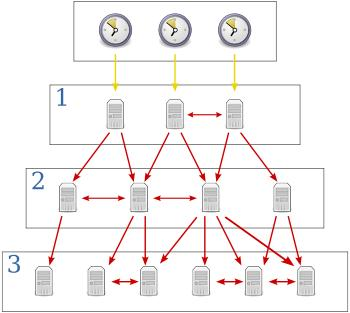
\includegraphics[scale=0.6, width=7cm]{fig/NTP1.jpg}
		\caption{Hierarquia no protocolo NTP}
		\end{center}
		\end{figure}
		
		O funcionamento do NTP consiste basicamente na troca de {\it timestamps} entre os servidores pertencentes a rede, estes {\it timestamps} são então utilizados para determinar os atrasos bidirecionais individuais, os {\it offsets} dos relógios e as estimativas de erros \cite{Mills1994}.
			
			
			\begin{figure}[ht]
				\begin{center}
				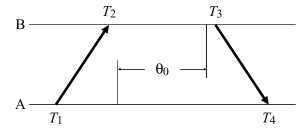
\includegraphics[scale=0.6, width=5cm]{fig/ntp3.jpg}
				\caption{{\it Timestamps} trocados pelo NTP \cite{Mills1994}}
				\end{center}
				\end{figure}
					
		De posse destas informações, há a necessidade de uma nova implementação do protocolo PTP, visto que o {\it daemon} proposto engloba a versão 1 do protocolo, enquanto que na versão 2 houveram melhorias, podendo citar a redução do tamanho da mensagem de sincronização, que facilita a sua implementação para sistemas embarcados. Além disso, o PTP permite obter um nível de precisão maior do que o obtido com o NTP \cite{DelRio2012}. 		
			
			
		%NTP timestamps are numbered and exchanged between peers A and B. Let T1, T2, T3, T4 be the values of the four most recent timestamps as shown and, without loss of generality, assume T3 > T2. Also, for the moment assume the clocks of A and B are stable and run at the same rate. Let
		%a = T2 − T1 and b = T3 − T4.
	%	If the network delay difference from A to B and from B to A, called differential delay, is small, % the clock offset θ and roundtrip delay δ of B relative to A at time T4 are close to
	%	θ = a + b 2
	%	and δ = a − b. (2)
	%	Each NTP message includes the latest three timestamps T1, T2 and T3, while the fourth T4 is determined upon arrival. Thus, both peers A and B can independently calculate delay and offset using a single bidirectional message stream. This is a symmetric, continuously sampled, time-transfer scheme similar to those used in some digital telephone networks
	%	B T2 T3
		
	% %	[LIN80]. Among its advantages are that errors due to missing or duplicated messages can be avoided.
	%	In [MIL92b] an exhaustive analysis is presented of the time and frequency errors that can accrue as the data are processed and refined at various levels in the subnet hierarchy. While the analysis is too long to repeat here, the results define the maximum error that can accrue under any operational condi- tion, called the synchronization distance λ, and the error expected under nominal operating conditions, called the dis- persion ε. There are several components of ε, including:
		%1. The maximum error in reading the local clock and each peer clock, which depends on the clock %resolution and method of adjustment.
		%2. The maximum error due to the frequency tolerance of the local clock and each peer clock since the time either was last set.
		%3. The estimated error contributed by each peer clock due to delay variations in the network and statistical latencies in the operating systems on the path to the primary reference source, which depends on differences between successive measurements for each peer clock. This is called the peer dispersion.
		%4. The estimated error contributed by the combined set of peers used to discipline the local clock, which depends upon the differences between individual members of the set. This is called the select dispersion.
	%	In practice, errors due to network delays usuually dominate ε. However, it is not possible to characterize these delays as a stationary random process, since network queues can grow and shrink in chaotic fashion and packet arrivals are fre- quently bursty. However, the method of calculating ε, as defined in the NTP Version 3 specification, represents a conservative estimate of the errors due to each of the above causes.
			
			
			
% ------------------------------------------------------------------------------


% ------------------------------------------------------------------------------
% ------------------------------------------------------------------------------
\section{DMEC} \label{dmec}
% + DMEC
% Describes the Distributed Motion Estimation Component (DMEC).
% Describes its parallelization Strategy (picture partition) as well the
% Coordinator-Worker model


% 1º parte independente de distribuído
% * Diagrama de classes: Interface PictureMotionEstimator                         (fig 3.1 relat tec): pme.dia
% Dizer que DMEC foi projetado seguindo os conceitos de ME.
% Engenharia de domínio da codificação de vídeo.
The Distributed Motion Estimation Component (DMEC) was developed following a
domain engineering process.
Before we explain how we have designed DMEC it is worth reviewing some
ME concepts from the domain of video encoding.
ME is a technique employed to explore the
similarity between neighboring pictures in a video sequence.
Figure \ref{fig:motion_estimation} illustrates the ME process for the neighboring
pictures \emph{A} and \emph{B}.
By searching for similarities between these two pictures, it is possible to determine
which blocks from picture \emph{A} are also found in picture \emph{B}.
Such displacement of picture blocks is encoded by \emph{motion vectors} 
(represented by the small arrows in the bottom side of
Figure \ref{fig:motion_estimation}).
Exploring the similarity between neighboring pictures allows for difference-based
encoding, thus increasing the compression rate of the generated 
bitstream \cite{citeulike:1269699}.

\fig{.4}{motion_estimation}{Motion Estimation}

Taking into consideration the concepts encompassed by the ME technique, we have
designed DMEC.
The central element of DMEC is described by the interface 
\emph{PictureMotionEstimator} shown by Figure \ref{fig:pme}.
Such interface describes entities that are responsible to perform ME of a whole
picture (or a partition of a picture).
An object of the type \emph{PictureMotionEstimator} knows all block modes of
the video standard in use (e.g. H.264), and works according to a specific
error metric, such as the Sum of Absolute Differences (SAD).
Such error metric is used to determine the similarity between neighboring
pictures.
The ME itself is computed by the \emph{match} method that takes the
current and the reference pictures
(respectively pictures \emph{A} and \emph{B} from Figure \ref{fig:motion_estimation})
and returns their ``counterpart'' which is composed by the motion vectors
and the motion cost.



% * Diagrama de classes: Retorno do match                                         (fig 3.2 relat tec): pmc.dia
% Dizer que retorna "tudo" é um componente bem auto contido.
DMEC was designed to be self contained, thus, the \emph{match} method computes ME
for all picture's macroblocks and for all block modes without any dependency
from another encoder element.
Therefore, the return of the method \emph{match}, which is conceptually shown
by Figure \ref{fig:pmc} is a multidimensional vector containing all motion
vectors and costs for each macroblock and block mode used in the ME.

\subsection{Parallelization Strategy}
% // DMEC: Parallelization Strategy //
% 2º parte distribuída
% * Figura particionamentos: todos os 6.                                          (TODO): picture_partition.XXX
% com ou sem o foreman. Pode ser sem, apenas retângulos.
% 
% * Figura threads/"atores" coordinator e workers                                 (from fig.git): dmec_thread_model-en.dia
% 
% * Diagrama de classes: módulos coordinator e workers                            (fig 3.4 relat tec): cnw.dia
% Motrar que vários algoritmos podem ser utilizados.


The parallelization strategy employed by DMEC is based on data partitioning,
in which the unit to be partitioned is the picture.
Figure \ref{fig:picture_partition} shows all picture partition modes available.
% It is worthy to mention that as all picture partitions dimensions must be 
% multiple to the macroblock dimension (16x16 pixels), it can occur having 
% partitions with distinct dimensions.
All picture partitions dimensions must be multiple to the macroblock dimension 
(16x16 pixels) to avoid having a macroblock broken between to neighboring
partitions.
If desired, it is possible to include new partition modes by specifying how the
partition should be performed.

% Fig showing all partitions types.
\fig{.2}{picture_partition}{Supported picture partitions modes}
% SINGLE_PARTITION = 1, 
% |0|
% 
% ONExTWO_PARTITION = 2,     
% |0|
% |1|
% 
% THREExONE_PARTITION = 3,
% |0|1|2|
% 
% TWOxTWO_PARTITION = 4,
% |0|1|
% |2|3|
% 
% THREE_TWOxTWO_PARTITION = 5,
% |0|1|2|
% |3 | 4|
% 
% THREExTWO_PARTITION = 6
% |0|1|2|
% |3|4|5|
% 

\fig{.4}{workers_and_bma}{Worker and Block Matching Algorithm}

In order to improve the performance of ME, each picture partition is then 
assigned to a \emph{Worker} module which executes in a specific functional unit,
such as a core of a multicore processor or a dedicated hardware element.
There is also a \emph{Coordinator} module, responsible to define the 
picture partition for each \emph{Worker} and to provide them with 
pictures to be processed.
The \emph{Coordinator} is also responsible to gather results generated by
\emph{Workers} (motion cost and motion vectors) and to deliver these results
back to the encoder. 
Figure \ref{fig:dmec_thread_model-en} illustrates the interaction
between the \emph{Coordinator} and \emph{Worker} modules.

\figtwocolumn{.4}{pme}{\emph{PictureMotionEstimator} interface}

% + Algoritmo
Each \emph{Worker} module computes ME by using a Block Matching Algorithm (BMA),
which itself also implements the \emph{PictureMotionEstimator} interface.
Thus, as shown by Figure \ref{fig:workers_and_bma}, all BMAs follow a single interface
therefore, it is possible to replace a BMA for another, according to the encoder
needs.

\subsection{Data Transference and Synchronization}
% // DMEC: Data Transference and Synchronization //
% * Diagrama de classes: TransferenceManager e SynchronizationManager             (TODO): dmec_trans_and_synch.dia
% Talvez seja um diagrama de sequencia até.
% 
% Mostrando como a transferencia de dados e sincronização são feitas.
% 
% É, diagrama de seq é bom.
% 
% Coordinator prepara pictures.
% Usa SynchronizationManager para Avisar que elas estão prontas (posso chamar de Barrier)
% Workers usam Transference Manager para obter as Pictures.
% Calculam ME e usar Transference Manager para divulgar os resultados
% Avisam Coordinator usando SynchronizationManager que o trabalho está pronto.
% 
% É meio um repeteco da figura thread model, mas é interessante para mostrar as
% interfaces de TransferenceManager e SynchronizationManager que serão implementadas
% pelo CELL, PC e Hardware...
The memory model used to exchange data between \emph{Coordinator} and
\emph{Worker} modules is a kind of shared memory, although, in practice, such
memory can be implemented as a memory block in a single address space 
(as is the case for our implementation for the IA32 architecture and
dedicated hardware), or
can be constituted by multiple memory blocks, each one using its own address
space
(as is the case for our implementation for the Cell BE architecture).

Figure \ref{fig:dmec_trans_and_synch} details the interaction between 
\emph{Coordinator} and \emph{Worker} modules.
At the beginning of the ME operation DMEC assumes that all pictures are in the
main memory.
Using the \emph{TransferenceManager} interface, \emph{Worker} modules can
obtain the samples of their picture partitions.
In the case of a memory block in a single address space, the operations of
\emph{TransferenceManager} are just pointer manipulations.
On the other hand, while using memory blocks in distinct address spaces, the
operations of \emph{TransferenceManager} are mapped to real 
memory transferences, such as Direct Memory Access (DMA) requisitions.
Also, by using the \emph{TransferenceManager}, \emph{Worker} modules 
can publish the computed motion vectors and motion costs.
% 
\emph{Worker} modules should wait for a signal from the \emph{Coordinator}
module indicating that there are pictures to the processed.
Similarly, the \emph{Coordinator} module should wait for the ME results 
generated by the \emph{Worker} modules.
Such synchronization operations are implemented by the 
\emph{SynchronizationManager} interface, which specifies barrier-like
mechanisms, which can be implemented using operating system operations or using
directly dedicated hardware elements.
In the case of a sequential operation with a single partition containing the
whole picture, the operations of \emph{SynchronizationManager} are canceled. 


% ------------------------------------------------------------------------------
% 
% Some notes
% DMEC Interfaces:
% 
% \emph{PictureMotionEstimator}
% 
% \emph{TransferenceManager}
% 
% \emph{SynchronizationManager}
% 
% 
% \emph{Coordinator} implements \emph{PictureMotionEstimator}
% 
% \emph{Worker} kind of implements \emph{PictureMotionEstimator}.
% The interface is other but it also performs match.
% The \emph{Worker} interface has a entry point ``run'', a match method,
% and some methods to gather the pictures and put the pictures back.
% 
% A \emph{Worker} uses the interfaces
% \emph{TransferenceManager} and \emph{SynchronizationManager}


% ------------------------------------------------------------------------------

% ------------------------------------------------------------------------------
% ------------------------------------------------------------------------------
\section{Practical Experiments} \label{eval}
% + Practical Experiments
% First shows speedup and quality results for DMEC
% using 1 (without partitioning) to 6 worker threads.
% Show that speedup is high and quality is kept acceptable.
% 
% Then, show speedup and quality results for DMEC integrated to JM and compares
%  to the original JM (and, if possible, to other works).
% 

% + JM
% + Dizer como realizamos os experimentos. E/ou quais as variáves observadas:
%   Evaluate the component in isolation DMEC to show its speedup.
%    And how it scales.
%   Evaluate the component in JM to show sppeedup and PSNR.
We have evaluated DMEC in two stages.
First, in order to verify how DMEC's performance scales from 
one to six \emph{Workers} instances, we have evaluated all DMEC implementations 
in a test case.
The test case application mimics the behavior of an H.264 encoder: it provides 
DMEC with pictures, obtain the ME results 
(motion vectors and motion cost), and checks if the results are correct.
Secondly, in order to assess DMEC influence on the final video quality, we have
evaluated all DMEC implementations in the
JM H.264 Reference Encoder~\cite{site:jm}.
The PSNR degradation is computed as the absolute PNSR difference between the
original encoder and the optimized ones.

% P: Dizer pq focamos em luma
For inter macroblock modes in H.264 (i.e. modes related to the ME),
the motion cost for chrominance components derives from the motion cost for 
luminance components~\cite{1101854}. 
Consequently the PSNR for chrominance components derives from the PSNR for 
luminance components. 
For this reason, in this paper we focus on the PSNR variation of the luminance 
component.

Figure \ref{fig:dmec-speedup_workers} show the speedup of DMEC in there
test case application with a different number of \emph{Workers} instances.
For such test, we have used an arbitrary set of pictures with a resolution of
1080p (Full-HD).
The speedup is normalized to one \emph{Worker} instance (speedup of 1X).

% TODO
% \textit{Comments about results in: Cell BE, Muticore IA32, and HW.}
It is worth to mention that for each number of \emph{Worker} instances
a different partition mode was used, according to
Figure \ref{fig:picture_partition}.
For one \emph{Worker} instance we have used the ``Single Partition'',
for two \emph{Worker} instances we have used the ``2x1'' partition and so on,
up to the ``2x3'' partition mode (used for six \emph{Worker} instances).

Besides the additional performance obtained by using a higher number of \emph{Worker} instances,
the partition mode also has influence on the speedup.
The reason of such influence is that, during the partitioning process, the dimensions of the
search window shrinks, thus reducing the area of the picture searched for
similarities.

\fig{.45}{dmec-speedup_workers}{Time performance scalability of DMEC}

% Sobre RD curves
% Figures XXX show the speedup of DMEC while tested already integrated to JM.
% The obtained values are compared to the ones obtained while using the original
% JM, without DMEC.
In order to evaluate in details the behavior of DMEC for distinct values 
of encoding bit-rates, we have used the BD-PSNR (Bjøntegaard Delta PSNR) metric
using the following values of QP (Quantization Parameter): 16,20,24,28; as 
described in \cite{gisle_bjntegaard_calculation_2001}.
It is important to evaluate quality (PSNR) for distinct bit-rates to test 
whether the approach can be used in distinct scenarios of application.
Figure \ref{fig:crowd-bitrate_psnr} shows the rate-distortions (RD) curves using the
original JM encoder and the optimized encoder using DMEC.
The video sequence used for this curves was \texttt{Crowd Run}, a 1080p sequence with  a
high ammount of motion.
Lower values of bit-rate are obtained for higher values of QP since by using
higher values for QP more data is discarded, thus increasing the
compression ratio. 
The two curves very near from each other indicates that the DMEC
presents a good rate-distortion performance for all the evaluated bit-rates.

\fig{.45}{crowd-bitrate_psnr}{RD curve of a 1080p video sequence}

We have evaluated also the speedup obtained in the
% encoding time
ME run time
while using
DMEC for the same QP values we used for BD-PSNR.
Figure \ref{fig:crowd-bitrate_speedup} shows the obtained values while using
6 \emph{Worker} instances.
For Muticore IA32, a speedup of around 9 times is obtained for all
bit-rate values.
For Cell BE this value is about 2 times.
A small speedup for the Cell BE, while compared to Multicore IA32 and the dedicated hardware, is due
to the memory transferences (picture samples and ME results) which is performed using
the DMA requisitions of Cell BE.


\fig{.45}{crowd-bitrate_speedup}{Speedup vs bit-rate of a 1080p sequence}
%
% \multfigtwov{.65}{bd_psnr}{bd_speedup} {bd} {RD curve (a) and speedup vs bit-rate (b) of 1080p sequence}

% Discussion


% Falar do paralelismo / particionamento de dados
% Qualidade ficou boa mesmo particionando e desempenho aumentou: speedup ~ 70%
%The strategy of ME distribution based on picture partitioning has been shown 
%effective.
% We have obtained a speedup higher than XXX\% without loosing quality.
%Data partitioning is effective because the visual interdependence between
%partitions is not significant to influence on the encoding quality, and allows
%for a speedup because it enables the simultaneous processing of each picture
%partition.

% - Falar da comunicação
% - Necessidade via espaço de endereçamentos diferentes
% A arquitetura Cell Broad Band demonstrou-se uma arquitetura interessante para o
% processamento paralelo de vídeo, pois possui unidades funcionais dedicadas 
% (i.e. SPEs) para processamento de dados. 
% A principal dificuldade encontrada em trabalhar-se com o Cell foi a capacidade 
% limitada da memória local das SPEs.
% Outra dificuldade foi lidar com as transferências de memória entre SPE e PPE. 
% Isto em fato foi superado pelas estratégias que desenvolvemos de baferização e 
% também com a utilização do Element Interconect Bus (EIB) do Cell que realiza 
% DMAs com altas taxas de transferências.
% 
% - Solução 1: Buffer de preditores, contribuiu bastante
% A estratégia de armazenamento de preditores nas SPEs foi significativa no 
% aumento do desempenho, pois vetores de movimentos necessários para o cálculo da
% ME não precisam ser consultados na memória principal. É coerente a decisão de 
% manter uma cópia local destes vetores, pois todos os vetores que a ME irá 
% precisar foram calculados pela partição em questão e por nenhuma outra.


% ------------------------------------------------------------------------------


% ------------------------------------------------------------------------------
% ------------------------------------------------------------------------------
\section{Conclusão} \label{concl}

Após realizarmos os testes concluímos a viabilidade da implementação do protocolo PTP para realizar a sincronização dos tempos de relógio em um sistema operacional embarcado, pois conseguimos manter o {\it offset} próximo a 0 segundo. Isso nos fornece uma base para trabalharmos a implementação com o intuito de obter um {\it offset} na faixa de sub-milissegundos. Obtendo essa precisão conseguiríamos garantir a aplicação, por exemplo, da implementação para sistemas de sensoriamento oceânico, como é abordado em \cite{DelRio2012}. Onde é feita uma abordagem sobre a implementação do protocolo PTP para distribuir os tempos de relógio em uma rede Ethernet de Sensoriamento Marinho(MSN). O fato da necessidade de um protocolo deste tipo para tal escopo se dá pelo fato de sinais GPS não estarem disponíveis devido à atenuação da água no fundo do mar e à requisitos de sincronização de instrumentos marítimos, tais como sismógrafos.




% ------------------------------------------------------------------------------

% if have a single appendix:
%\appendix[Proof of the Zonklar Equations]
% or
%\appendix  % for no appendix heading
% do not use \section anymore after \appendix, only \section*
% is possibly needed

% use appendices with more than one appendix
% then use \section to start each appendix
% you must declare a \section before using any
% \subsection or using \label (\appendices by itself
% starts a section numbered zero.)
%


% \appendices
% \section{Proof of the First Zonklar Equation}
% Appendix one text goes here.
% 
% % you can choose not to have a title for an appendix
% % if you want by leaving the argument blank
% \section{}
% Appendix two text goes here.


% use section* for acknowledgement

% TODO colocar número do projeto.
% PROJETO: INF/FINEP 01.08.0287.00-REDEH264
% NÚMERO:
% 06341 - X



% Can use something like this to put references on a page
% by themselves when using endfloat and the captionsoff option.
\ifCLASSOPTIONcaptionsoff
  \newpage
\fi



% trigger a \newpage just before the given reference
% number - used to balance the columns on the last page
% adjust value as needed - may need to be readjusted if
% the document is modified later
%\IEEEtriggeratref{8}
% The "triggered" command can be changed if desired:
%\IEEEtriggercmd{\enlargethispage{-5in}}

% references section

% can use a bibliography generated by BibTeX as a .bbl file
% BibTeX documentation can be easily obtained at:
% http://www.ctan.org/tex-archive/biblio/bibtex/contrib/doc/
% The IEEEtran BibTeX style support page is at:
% http://www.michaelshell.org/tex/ieeetran/bibtex/
%\bibliographystyle{IEEEtran}
% argument is your BibTeX string definitions and bibliography database(s)
%\bibliography{IEEEabrv,../bib/paper}
%
% <OR> manually copy in the resultant .bbl file
% set second argument of \begin to the number of references
% (used to reserve space for the reference number labels box)
% References
\bibliographystyle{IEEEtran}
\bibliography{referencia}


\end{document}
